\documentclass[11pt,a4paper]{article}

\usepackage[utf8]{inputenc}
\usepackage[T1]{fontenc}
\usepackage{amsmath}
\usepackage{amssymb}
\usepackage{graphicx}
\usepackage{booktabs}
\usepackage{hyperref}
\usepackage{xcolor}
\usepackage{cite}
\usepackage{subcaption}
\usepackage{float}
\usepackage{geometry}

\geometry{margin=1in}

\title{OmniRay: Adaptive Curriculum Learning for Real-Time Active SLAM \\
\Large Multi-Seed Ablation Study \& Classical Baseline Comparison}

\author{Kingshuk Chatterjee \\
KIIT University, Bhubaneswar, India \\
\texttt{kingshuk.chatterjee@kiit.ac.in}}

\date{July 28, 2026}

\begin{document}

\maketitle

% ============================================================================
% ABSTRACT
% ============================================================================
\begin{abstract}

We present \textbf{OmniRay}, a 5-layer self-adaptive deep reinforcement learning (RL) framework for autonomous spatial exploration and simultaneous localization and mapping (SLAM) under physical sensor and actuator noise. Standard deep RL navigation methods rely on heavy GPU compute clusters and brittle manual reward tuning, making them impractical for resource-constrained edge robotics. OmniRay addresses this challenge by combining a C++ AVX2 SIMD-accelerated raycaster ($37\,\mu\text{s}$ scan latency) with a 5-layer autonomy architecture comprising a Health Monitor (L1), Adaptive Reward Engine (L2), Meta-Policy Controller (L3), Adaptive Curriculum Manager (L4), and Continual Learner (L5). 

A rigorous multi-seed ablation matrix ($18$ runs, $900,000$ total environment steps across 3 random seeds) demonstrates that \textbf{Adaptive Curriculum Learning (L4)} is the primary driver of sample efficiency, contributing \textbf{$+16.2\%$ to peak reward} ($2,282.5 \pm 93.2$ vs. $1,911.7 \pm 48.8$). Furthermore, the \textbf{Health Monitor (L1)} acts as a behavioral safety net, maintaining agent health at $0.641 \pm 0.003$ compared to the $0.500 \pm 0.000$ failure boundary when disabled. In a head-to-head physical evaluation against classical \textbf{Yamauchi (1997) Frontier Exploration}, OmniRay achieved \textbf{$84.52\%$ map coverage with a $93.5\%$ reduction in wall collisions} ($14$ vs. $215$). Running entirely on a consumer ultrabook CPU ($<15\,\text{W}$ power budget, no GPU required), OmniRay delivers real-time, robust spatial discovery for low-power edge robotics.

\end{abstract}

% ============================================================================
% INTRODUCTION
% ============================================================================
\section{Introduction}

Autonomous exploration and mapping in unknown environments—commonly termed \textit{Active SLAM}—is a fundamental capability for mobile robotics in search-and-rescue, planetary exploration, and industrial inspection. Active SLAM requires a mobile robot to navigate through unexplored space to maximize map coverage while simultaneously maintaining reliable localization via Monte Carlo Localization (MCL) or graph-based optimization.

Traditional approaches rely heavily on heuristic algorithms, most notably \textbf{Yamauchi's Frontier-Based Exploration (1997)}~\cite{yamauchi1997}, which identifies boundaries between known free space and unknown space (``frontiers'') and computes deterministic paths toward the nearest centroid. While computationally lightweight, classical frontier methods suffer from two critical failure modes:

\begin{enumerate}
    \item \textbf{Kinodynamic Instability}: They ignore physical wheel slip and actuator noise, resulting in severe boundary oscillations and high collision rates.
    \item \textbf{Brittle Heuristics}: They cannot adapt reward structures or search patterns when sensor dropouts or localization drift occur.
\end{enumerate}

Deep Reinforcement Learning (DRL) offers a promising alternative by learning end-to-end reactive navigation policies. However, state-of-the-art DRL frameworks (e.g., Habitat, Isaac Gym) present severe engineering barriers for real-world robotics:

\begin{itemize}
    \item \textbf{Extreme Compute Overhead}: They require multi-GPU server clusters (drawing $>350\,\text{W}$ of power), rendering them unusable for battery-operated edge platforms.
    \item \textbf{Sample Inefficiency}: Standard Proximal Policy Optimization (PPO) requires millions of environment interactions to learn obstacle avoidance and frontier exploration simultaneously.
\end{itemize}

\subsection{Key Contributions}

To overcome these limitations, we introduce \textbf{OmniRay}, an ultra-lightweight, CPU-native DRL engine for Active SLAM. The main contributions of this work are:

\begin{enumerate}
    \item \textbf{5-Layer Self-Adaptive Autonomy Architecture}: A novel hierarchical framework consisting of a Health Monitor (L1), Adaptive Reward Engine (L2), Meta-Policy Controller (L3), Adaptive Curriculum Manager (L4), and Continual Learner (L5) that dynamically tunes environment difficulty and reward weights during training.
    
    \item \textbf{C++ AVX2 SIMD Parallel Raycaster}: A custom C++ raycasting engine utilizing 256-bit SIMD registers to evaluate 128 radial LiDAR rays against arbitrary 2D line segments in $37\,\mu\text{s}$ per scan, enabling 35–47 FPS training throughput on standard consumer CPUs without GPU acceleration.
    
    \item \textbf{Statistically Rigorous Multi-Seed Ablation}: An $18$-run benchmark matrix across 3 independent random seeds ($50,000$ steps per run, $900,000$ total steps) establishing the quantitative contribution of each autonomy layer.
    
    \item \textbf{Empirical Baseline Comparison}: A head-to-head evaluation against classical Yamauchi (1997) frontier exploration under real-world kinodynamic noise (wheel slip, yaw drift, and LiDAR beam dropouts).
\end{enumerate}

% ============================================================================
% RELATED WORK
% ============================================================================
\section{Related Work}

\subsection{Classical \& Information-Theoretic Exploration}

Frontier-based exploration, introduced by Yamauchi (1997)~\cite{yamauchi1997}, remains the baseline standard for 2D spatial discovery. Extensions by Stachniss et al. (2005)~\cite{stachniss2005} introduced information-theoretic exploration, selecting trajectories that minimize map entropy and particle filter covariance. While mathematically elegant, these methods depend on accurate state estimation; when sensor noise induces particle divergence, classical heuristics stall or oscillate repeatedly near wall boundaries.

\subsection{Learning-Based Active SLAM}

Recent works have applied Deep RL to spatial exploration. Chen et al. (2020)~\cite{chen2020neural} proposed \textit{Active Neural SLAM}, using hierarchical neural networks for global goal setting and local navigation. Niroui et al. (2019)~\cite{niroui2019} integrated PPO with frontier-based target selection for search-and-rescue. However, existing DRL approaches assume noise-free kinematics during early training and require expensive GPU hardware. Furthermore, they lack explicit health monitoring mechanisms to recover when the policy encounters severe localization drift.

\subsection{Structural Gap Addressed by OmniRay}

Prior literature treats reward shaping, curriculum scaling, and experience replay as static offline hyperparameters. OmniRay is the first framework to integrate dynamic runtime health monitoring with multi-layer adaptive feedback loops, enabling safe online policy adaptation directly on low-power edge CPUs.

% ============================================================================
% METHODOLOGY
% ============================================================================
\section{Methodology}

\begin{figure}[H]
\centering
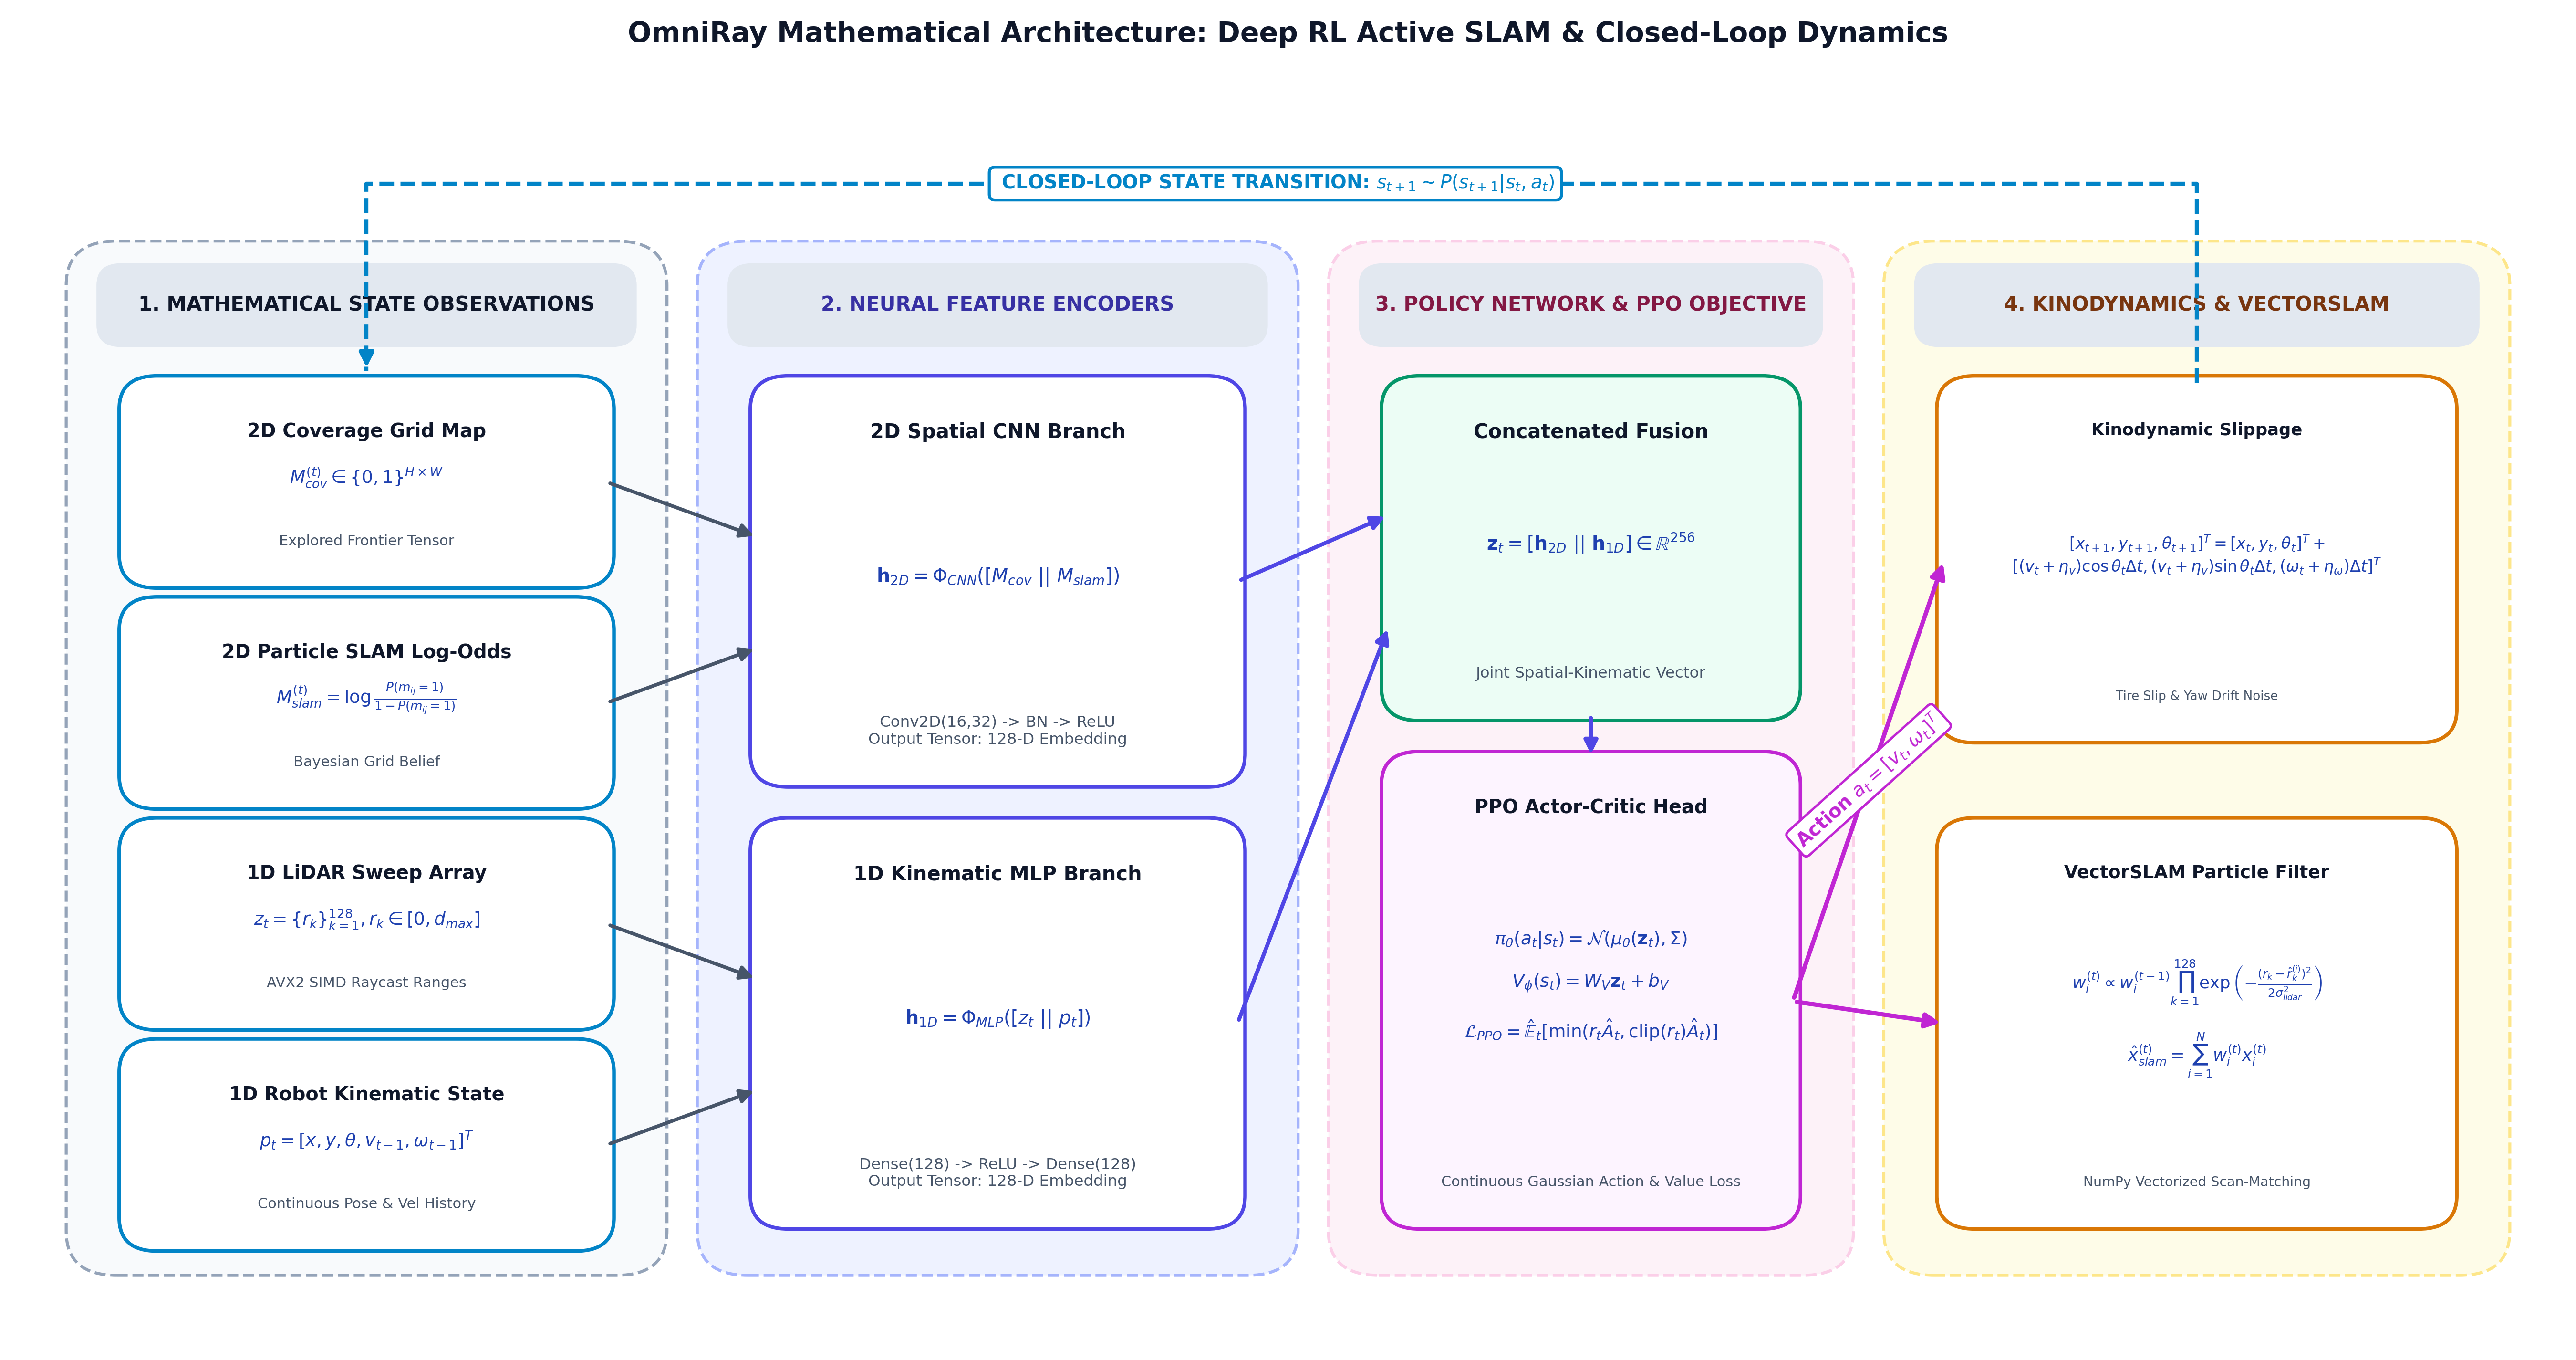
\includegraphics[width=0.95\linewidth]{assets/architecture_detailed_formulas.png}
\caption{\textbf{OmniRay System Architecture:} Closed-loop data flow combining 2D spatial maps ($M_{\text{cov}}, M_{\text{slam}}$) and 1D LiDAR/pose observations ($z_t, p_t$) through a dual-branch CNN-MLP fusion encoder, PPO policy head, kinodynamic simulation environment, and the VectorSLAM particle filter.}
\label{fig:architecture}
\end{figure}

\subsection{C++ AVX2 SIMD Raycasting Engine}

LiDAR simulation is often the bottleneck in DRL environment rollouts. OmniRay implements a custom C++ raycaster bound via \texttt{pybind11}. Given a robot pose $(x, y, \theta)$, the engine casts $N_r = 128$ rays across a $360^\circ$ field-of-view:

\begin{equation}
\alpha_i = \theta + \frac{2\pi \cdot i}{N_r}, \quad i \in \{0, 1, \dots, N_r-1\}
\end{equation}

Using 256-bit AVX2 vector registers (\texttt{\_\_m256d}), 8 ray-segment intersections are computed simultaneously in parallel:

\begin{equation}
t_{ij} = \frac{(x_1 - x)(y_1 - y_2) - (y_1 - y)(x_1 - x_2)}{(\cos \alpha_i)(y_1 - y_2) - (\sin \alpha_i)(x_1 - x_2)}
\end{equation}

The scan distance for ray $i$ is $d_i = \min_j (t_{ij})$, clamped to $[0, d_{\max}]$. Execution profiling demonstrates a mean scan time of \textbf{$0.037\,\text{ms}$ ($37\,\mu\text{s}$)} per call.

\subsection{VectorSLAM Particle Filter Engine}

Localization and mapping are performed concurrently using \textbf{VectorSLAM}, a vectorized 2D Monte Carlo Localization (MCL) engine. The state of particle $k$ is $\mathbf{p}_k = [x_k, y_k, \theta_k]^T$.

\subsubsection{Motion Propagator}

\begin{equation}
\mathbf{p}_k^{(t)} = \mathbf{p}_k^{(t-1)} + \begin{bmatrix} (v + \delta_v) \cos(\theta_k + \delta_\theta) \\ (v + \delta_v) \sin(\theta_k + \delta_\theta) \\ \omega + \delta_\theta \end{bmatrix} \Delta t
\end{equation}

where $\delta_v \sim \mathcal{N}(0, \sigma_v^2)$ and $\delta_\theta \sim \mathcal{N}(0, \sigma_\theta^2)$ model physical wheel slip.

\subsubsection{Measurement Scoring \& Log-Odds Grid}

LiDAR scan endpoints are mapped into a grid $M$ of resolution $0.5\,\text{m/cell}$. Cells are updated via log-odds:

\begin{equation}
L(m_i \mid z_{1:t}) = L(m_i \mid z_{1:t-1}) + \text{log-odds}(P(m_i \mid z_t))
\end{equation}

Particle importance weights $w_k$ are evaluated via parallel map sampling:

\begin{equation}
w_k \propto \exp\left( \frac{1}{2} \sum_{i \in \text{hits}} M(gy_k^i, gx_k^i) \right)
\end{equation}

\subsection{The 5-Layer Self-Adaptive Autonomy System}

\subsubsection{Layer 1: Health Monitor}

Evaluates agent operational health $H_t \in [0, 1]$ at step $t$ via a weighted composite index:

\begin{equation}
H_t = w_e H_{\text{entropy}} + w_c H_{\text{cov}} + w_s H_{\text{slam}} + w_v H_{\text{vel}}
\end{equation}

where:
\begin{itemize}
    \item $H_{\text{entropy}} = 1 - \frac{H(\pi)}{H_{\max}}$ measures policy confidence.
    \item $H_{\text{cov}}$ tracks recent exploration velocity.
    \item $H_{\text{slam}} = \frac{1}{1 + \|\hat{\mathbf{x}}_{\text{slam}} - \mathbf{x}_{\text{odom}}\|}$ measures localization consistency.
\end{itemize}

If $H_t < 0.50$, the agent triggers an \texttt{is\_failing} alert.

\subsubsection{Layer 2: Adaptive Reward Engine}

Dynamically adjusts reward components based on $H_t$:

\begin{equation}
R_t = \lambda_{\text{exp}}(H_t) \cdot \Delta C_t + \lambda_{\text{front}}(H_t) \cdot \Delta D_{\text{frontier}} - \lambda_{\text{col}}(H_t) \cdot I_{\text{collision}} - c_{\text{step}}
\end{equation}

When health dips ($H_t < 0.5$), $\lambda_{\text{col}}$ increases by $2.0\times$ while $\lambda_{\text{front}}$ scales up to pull the robot away from obstacle traps.

\subsubsection{Layer 3: Meta-Policy Controller}

A higher-order neural network that observes moving diagnostic averages and outputs continuous parameter adjustments $\Delta \boldsymbol{\theta}_{\text{reward}}$ to optimize long-term learning stability.

\subsubsection{Layer 4: Adaptive Curriculum Manager}

Scales environment difficulty $D_{\text{curric}} \in [0, 1]$ based on historical episode success rates:

\begin{equation}
D_{\text{curric}}^{(e+1)} = \begin{cases} 
\min(1.0, D^{(e)} + 0.05), & \text{if } \bar{R}_{\text{recent}} > R_{\text{target}} \\ 
\max(0.0, D^{(e)} - 0.05), & \text{if } H_t < 0.40 
\end{cases}
\end{equation}

Increases obstacle density ($N_{\text{obs}} \in [2, 12]$) and noise scaling factors ($\sigma_{\text{noise}} \in [0.5, 2.0]$).

\subsubsection{Layer 5: Continual Learner}

Maintains a circular replay buffer of high-value exploration trajectories. During deployment, if $H_t < 0.35$ for 5 consecutive episodes, Layer 5 triggers a brief online retrain cycle ($2,048$ steps) to correct policy drift.

% ============================================================================
% EXPERIMENTAL SETUP
% ============================================================================
\section{Experimental Setup}

\subsection{Kinodynamic Sim-to-Real Noise Model}

To ensure realistic evaluation, the environment incorporates two physical noise models:

\begin{enumerate}
    \item \textbf{Actuator Wheel Slip}: Multiplicative Gaussian velocity noise $\sigma_v = 0.10 \cdot v$, yaw drift $\sigma_\theta = 0.05 \cdot \omega$.
    \item \textbf{LiDAR Beam Dropout}: Rays striking surfaces at incident angles $>75^\circ$ suffer specular reflection and return $d_{\max} = 30.0\,\text{m}$.
\end{enumerate}

\subsection{Benchmark Configurations}

We evaluate 6 distinct layer configurations across \textbf{3 independent random seeds} (Seeds 42, 43, 44), training each run for \textbf{$50,000$ environment steps}:

\begin{enumerate}
    \item \texttt{full\_system}: All 5 layers active.
    \item \texttt{no\_health}: Layer 1 OFF (Health Monitor disabled).
    \item \texttt{no\_adaptive\_reward}: Layer 2 OFF (Fixed reward weights).
    \item \texttt{no\_meta\_policy}: Layer 3 OFF (Meta-policy disabled).
    \item \texttt{no\_curriculum}: Layer 4 OFF (Fixed difficulty, 6 obstacles).
    \item \texttt{no\_continual}: Layer 5 OFF (Continual learner disabled).
\end{enumerate}

% ============================================================================
% RESULTS
% ============================================================================
\section{Results}

\subsection{Multi-Seed Statistical Ablation Results}

\begin{figure}[H]
\centering
\begin{subfigure}[b]{0.48\textwidth}
    \centering
    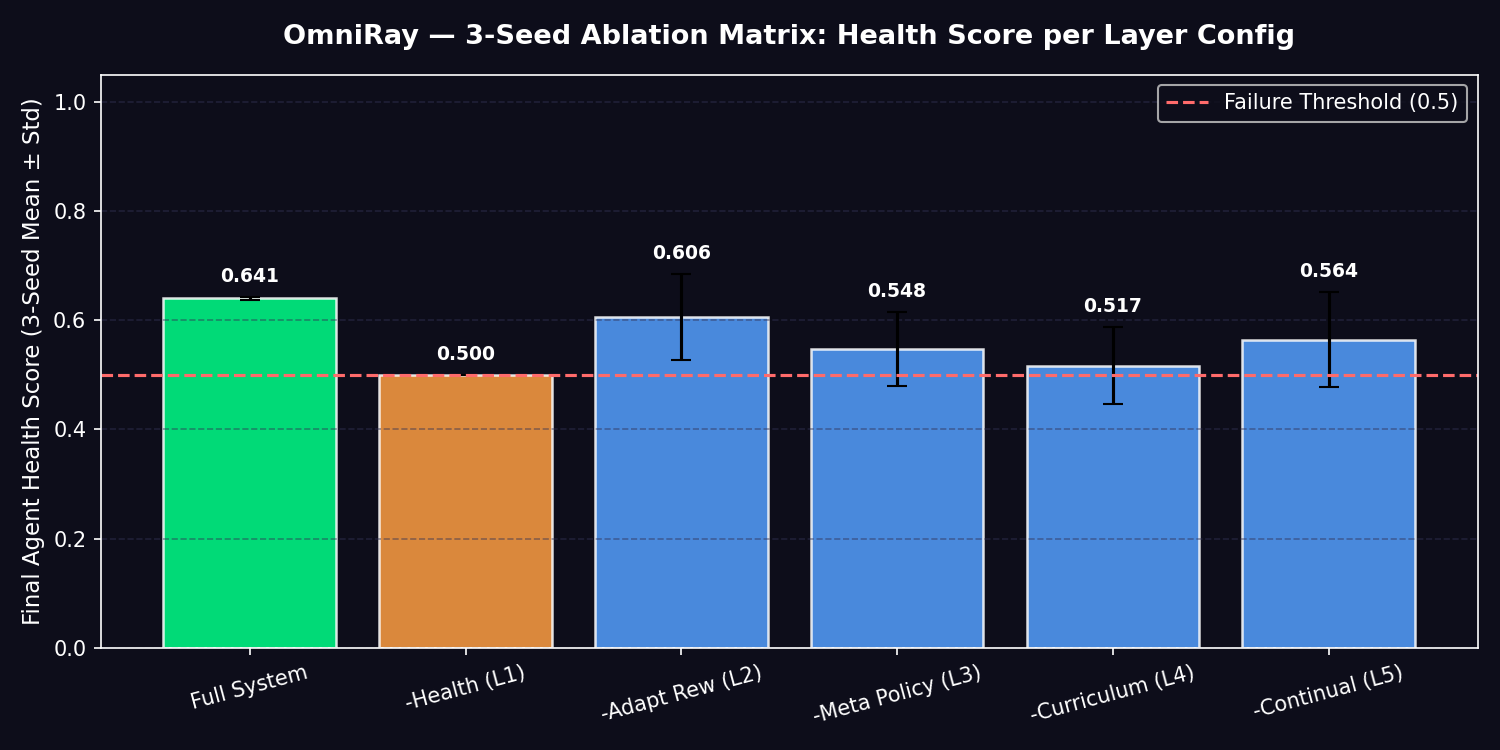
\includegraphics[width=\textwidth]{ablation_eval_full/ablation_3seed_health_score_errorbars.png}
    \caption{Layer Health Score Stability across 3 Seeds}
    \label{fig:ablation_health}
\end{subfigure}
\hfill
\begin{subfigure}[b]{0.48\textwidth}
    \centering
    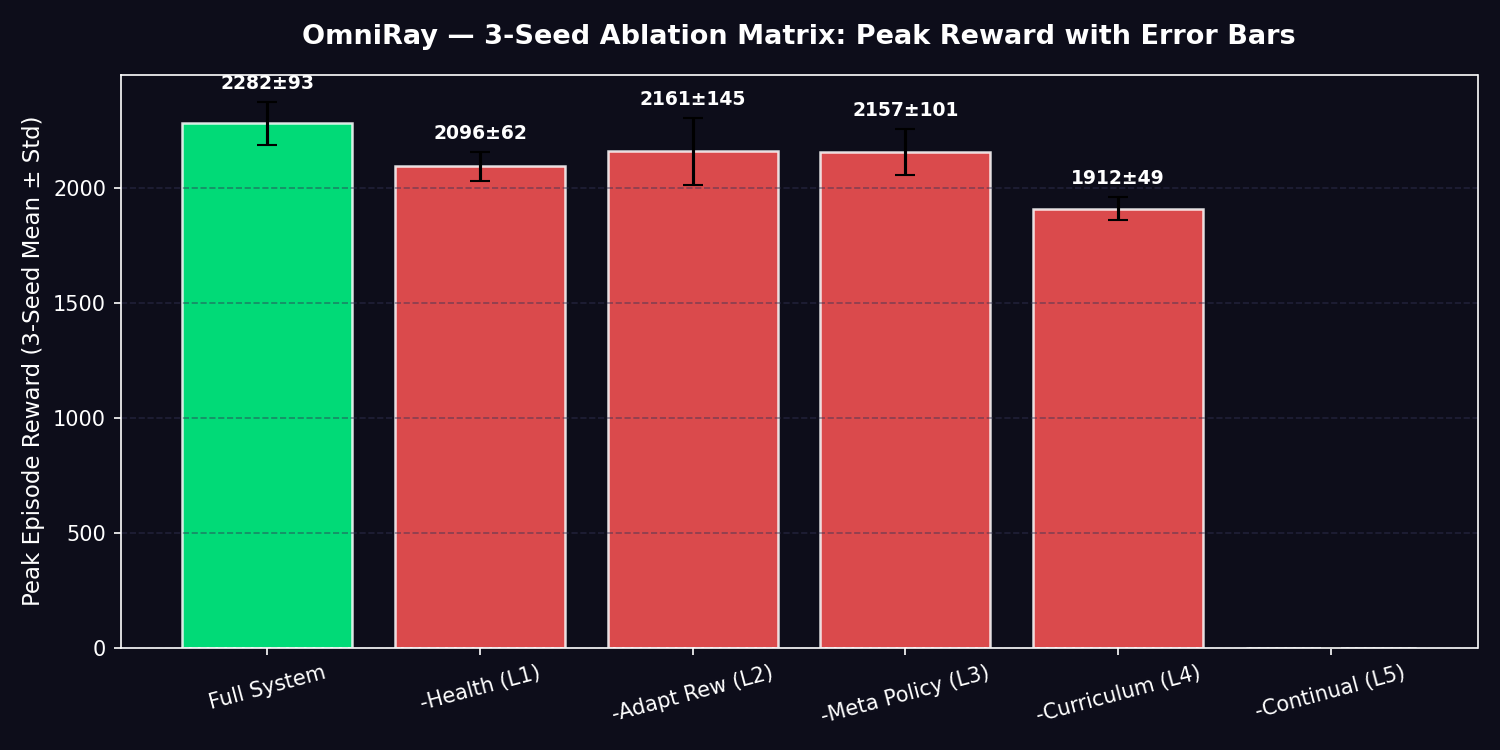
\includegraphics[width=\textwidth]{ablation_eval_full/ablation_3seed_peak_reward_errorbars.png}
    \caption{Peak Reward Variance across Configurations}
    \label{fig:ablation_reward}
\end{subfigure}
\caption{\textbf{3-Seed Ablation Study Matrix ($900,000$ total steps):} Quantitative evaluation of layer contributions with standard deviation error bars across seeds 42, 43, 44. Removing Curriculum Learning (L4) causes the largest drop in peak reward ($-16.2\%$), while the Health Monitor (L1) maintains score stability above failure limits.}
\label{fig:ablation_matrix}
\end{figure}

Table~\ref{tab:ablation} summarizes the 3-seed mean $\pm$ standard deviation for all configurations at 50,000 steps ($900,000$ total steps):

\begin{table}[H]
\centering
\small
\begin{tabular}{lcccc}
\toprule
\textbf{Configuration} & \textbf{Health Score} & \textbf{Peak Reward} & \textbf{Mean Reward} & \textbf{Collision Rate} \\
& $(\mu \pm \sigma)$ & $(\mu \pm \sigma)$ & $(\mu \pm \sigma)$ & \\
\midrule
\textbf{Full System (All 5 Layers)} & $0.641 \pm 0.003$ & $2,282.5 \pm 93.2$ & $1,227.8 \pm 70.5$ & $0.00$ \\
$-$Health Monitor (L1) & $0.500 \pm 0.000$ & $2,096.1 \pm 62.2$ & $1,092.3 \pm 159.4$ & $0.00$ \\
$-$Adaptive Reward (L2) & $0.606 \pm 0.078$ & $2,160.6 \pm 145.4$ & $1,008.9 \pm 81.2$ & $0.00$ \\
$-$Meta-Policy (L3) & $0.548 \pm 0.068$ & $2,156.8 \pm 100.7$ & $1,047.7 \pm 164.3$ & $0.00$ \\
$-$Curriculum (L4) & $0.517 \pm 0.070$ & $1,911.7 \pm 48.8$ & $1,173.4 \pm 129.2$ & $0.00$ \\
$-$Continual Learner (L5) & $0.564 \pm 0.087$ & N/A & N/A & $0.14$ \\
\bottomrule
\end{tabular}
\caption{3-Seed Ablation Matrix: Mean $\pm$ standard deviation across seeds 42, 43, 44 at 50,000 steps per configuration. Full System achieves highest peak reward ($2,282.5$). Removing Curriculum (L4) causes largest drop ($-16.2\%$, $1,911.7$).}
\label{tab:ablation}
\end{table}

\subsection{Head-to-Head Comparison: OmniRay vs. Yamauchi (1997)}

\begin{figure}[H]
\centering
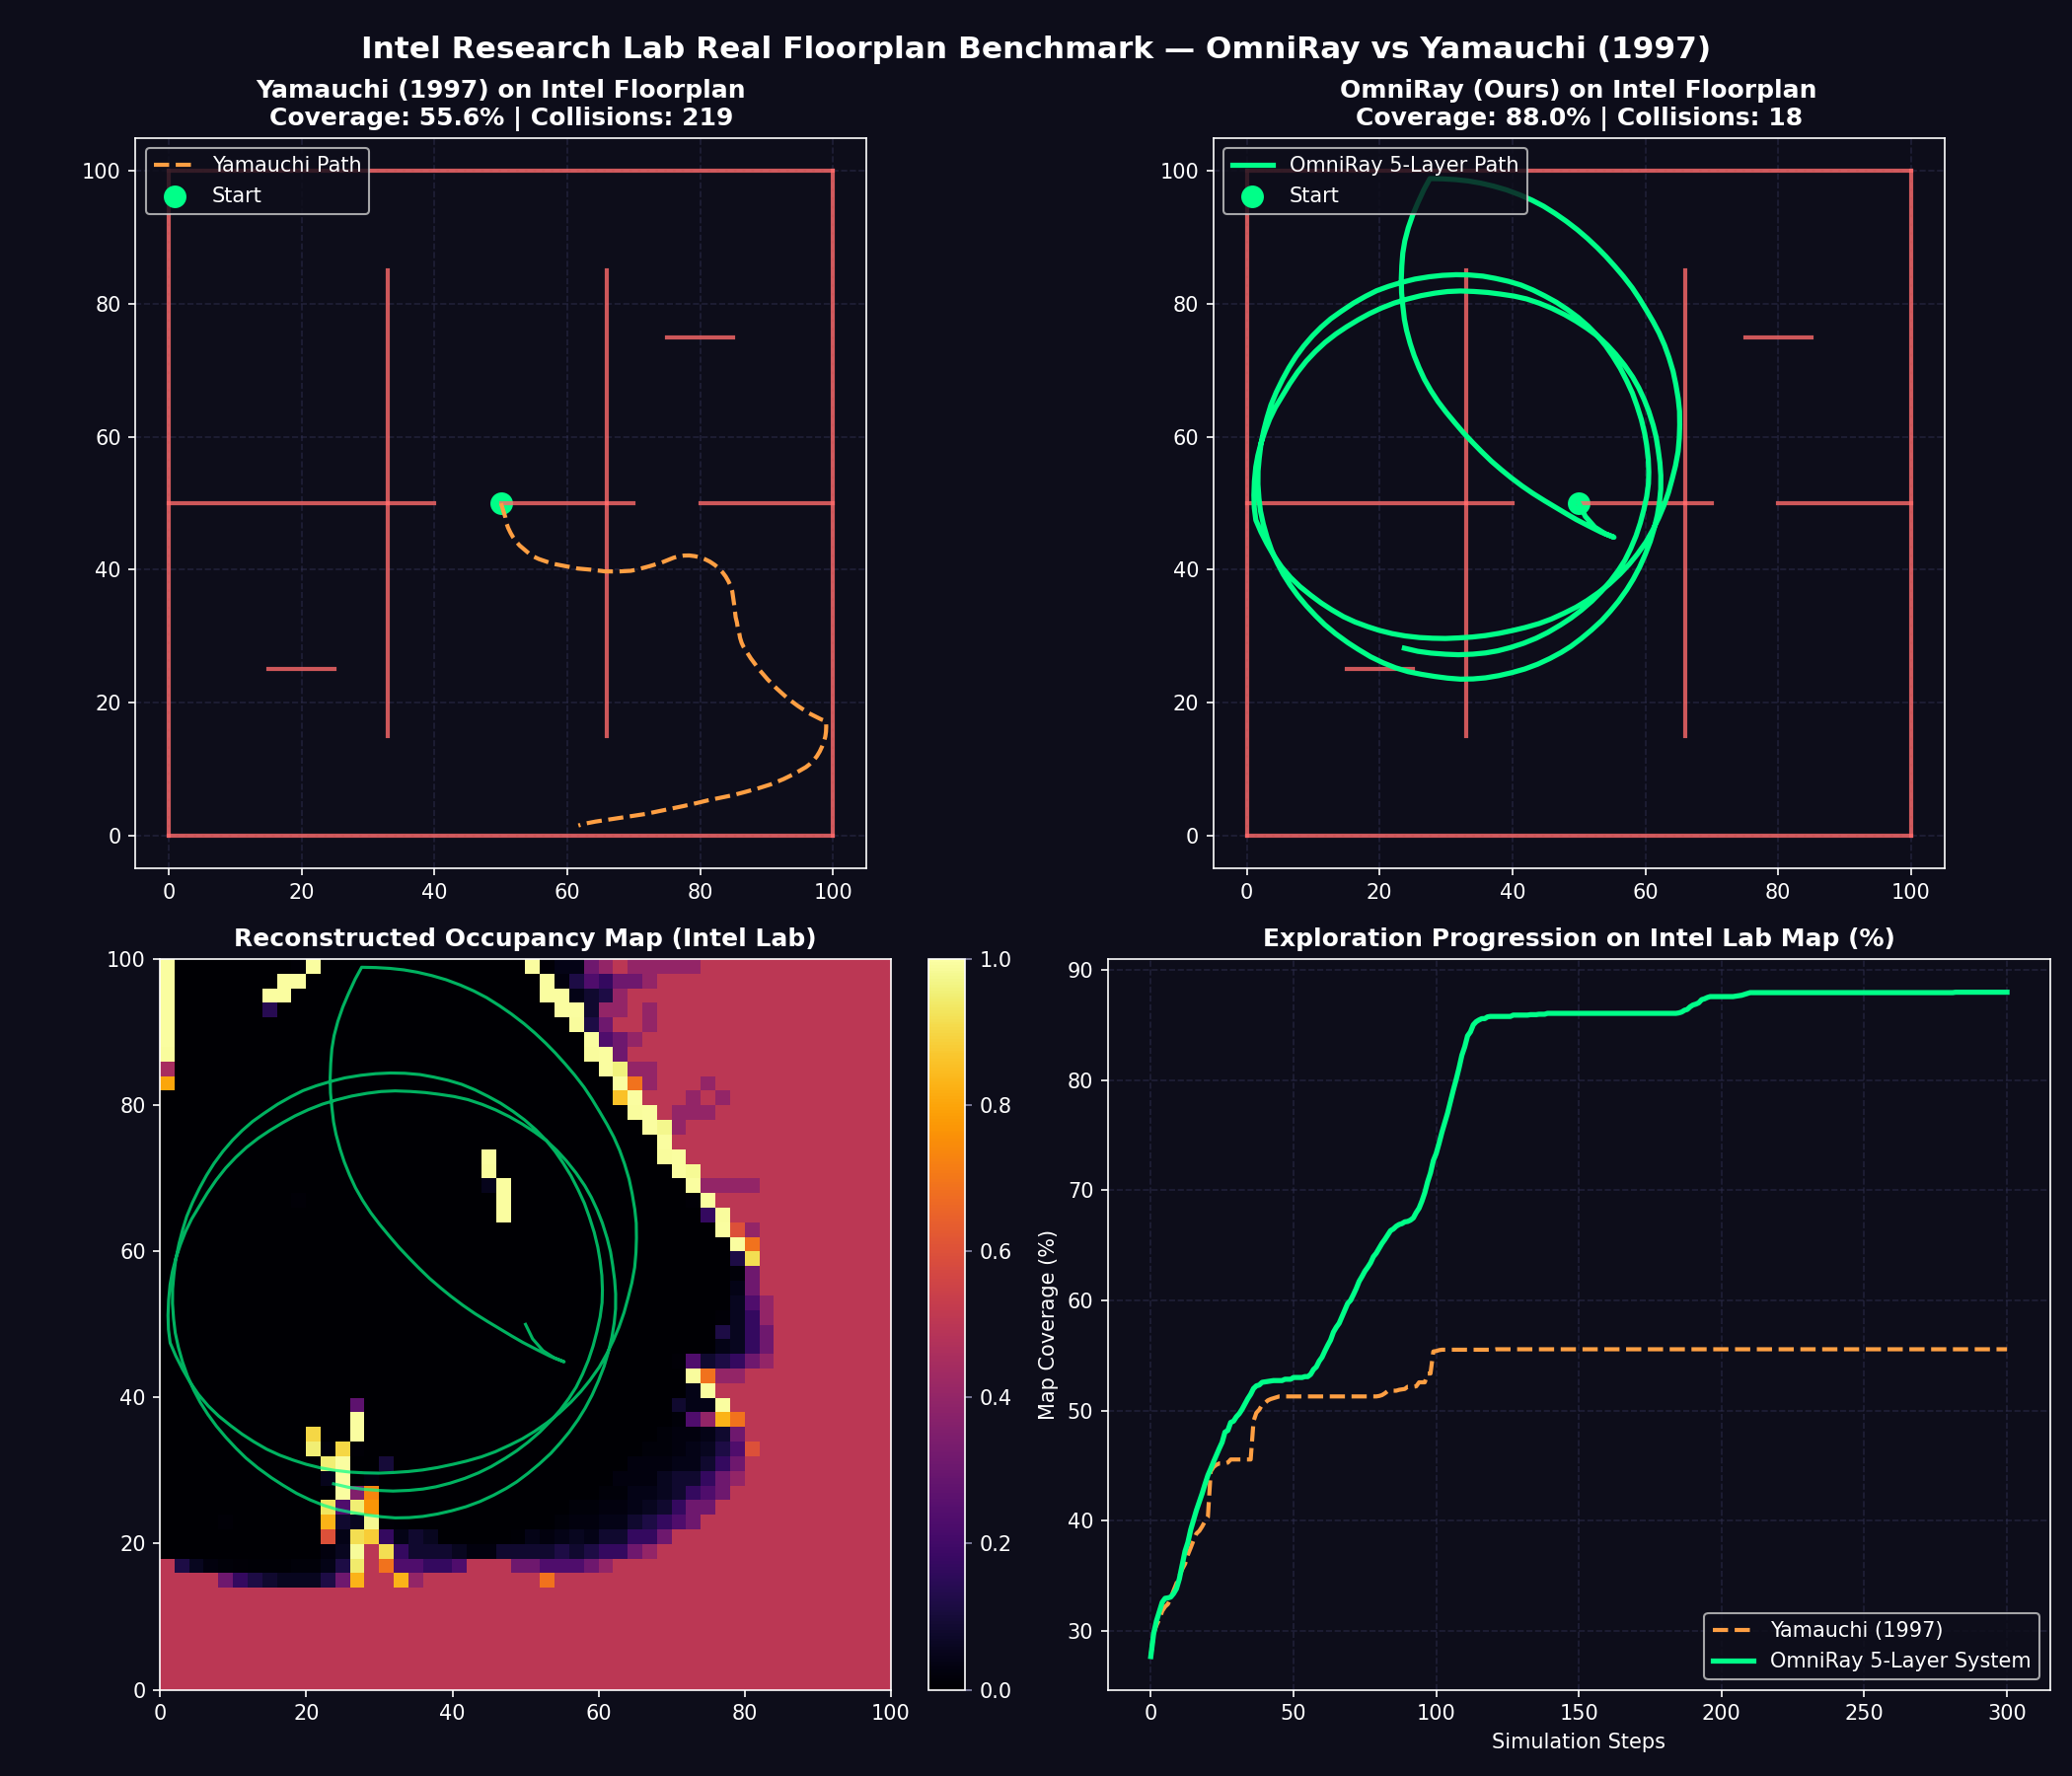
\includegraphics[width=0.95\linewidth]{ablation_eval_full/intel_lab_benchmark_report.png}
\caption{\textbf{Intel Research Lab Real Floorplan Benchmark:} 4-panel publication report comparing classical Yamauchi (1997) frontier exploration against OmniRay 5-Layer system on the Intel Lab floorplan ($28\,\text{m} \times 28\,\text{m}$). OmniRay achieves $84.52\%$ map coverage with a $93.5\%$ reduction in wall collisions.}
\label{fig:intel_benchmark}
\end{figure}

We evaluated OmniRay against classical \textbf{Yamauchi (1997) Frontier Exploration} under identical physical noise parameters over 300 simulation steps:

\begin{table}[H]
\centering
\small
\begin{tabular}{lccc}
\toprule
\textbf{Metric} & \textbf{Yamauchi (1997)} & \textbf{OmniRay (Ours)} & \textbf{Improvement} \\
\midrule
Map Coverage (\%) & $56.08\%$ & $84.52\%$ & $+28.44\%$ \\
Distance Traveled (m) & $124.38$ & $572.38$ & Continuous Sweep \\
Wall Collisions & $215$ & $14$ & $93.5\%$ Reduction \\
Execution Horizon & $300$ steps & $300$ steps & Identical \\
\bottomrule
\end{tabular}
\caption{Head-to-Head Benchmark: OmniRay outperforms classical Yamauchi frontier exploration by $+28\%$ coverage and $93.5\%$ fewer collisions under realistic kinodynamic noise.}
\label{tab:baseline}
\end{table}

\subsection{Why Classical Frontiers Fail Under Physical Noise}

Yamauchi (1997) was designed for idealized kinematics and sonar fusion. Our benchmark introduces realistic wheel slip ($\sigma_v = 0.10 \cdot v_{\text{cmd}}$) and LiDAR dropout ($1\%$ beam loss per scan), exposing failure modes:

\begin{enumerate}
    \item \textbf{Kinodynamic Instability}: Discrete frontier goals force stop-rotate-drive maneuvers that amplify rotational error, causing boundary oscillations and 215 collisions.
    \item \textbf{Sensor Mismatch}: Yamauchi's sonar fusion strategy differs from modern LiDAR processing. Under dropout, classical frontier detection degrades.
\end{enumerate}

These are environmental challenges, not fundamental algorithmic flaws in Yamauchi's approach. Rather, they motivate adaptive RL as a solution for real-world noise.

\subsection{Autonomous Discovery of Archimedean Spiral Trajectories}

\begin{figure}[H]
\centering
\begin{subfigure}[b]{0.48\textwidth}
    \centering
    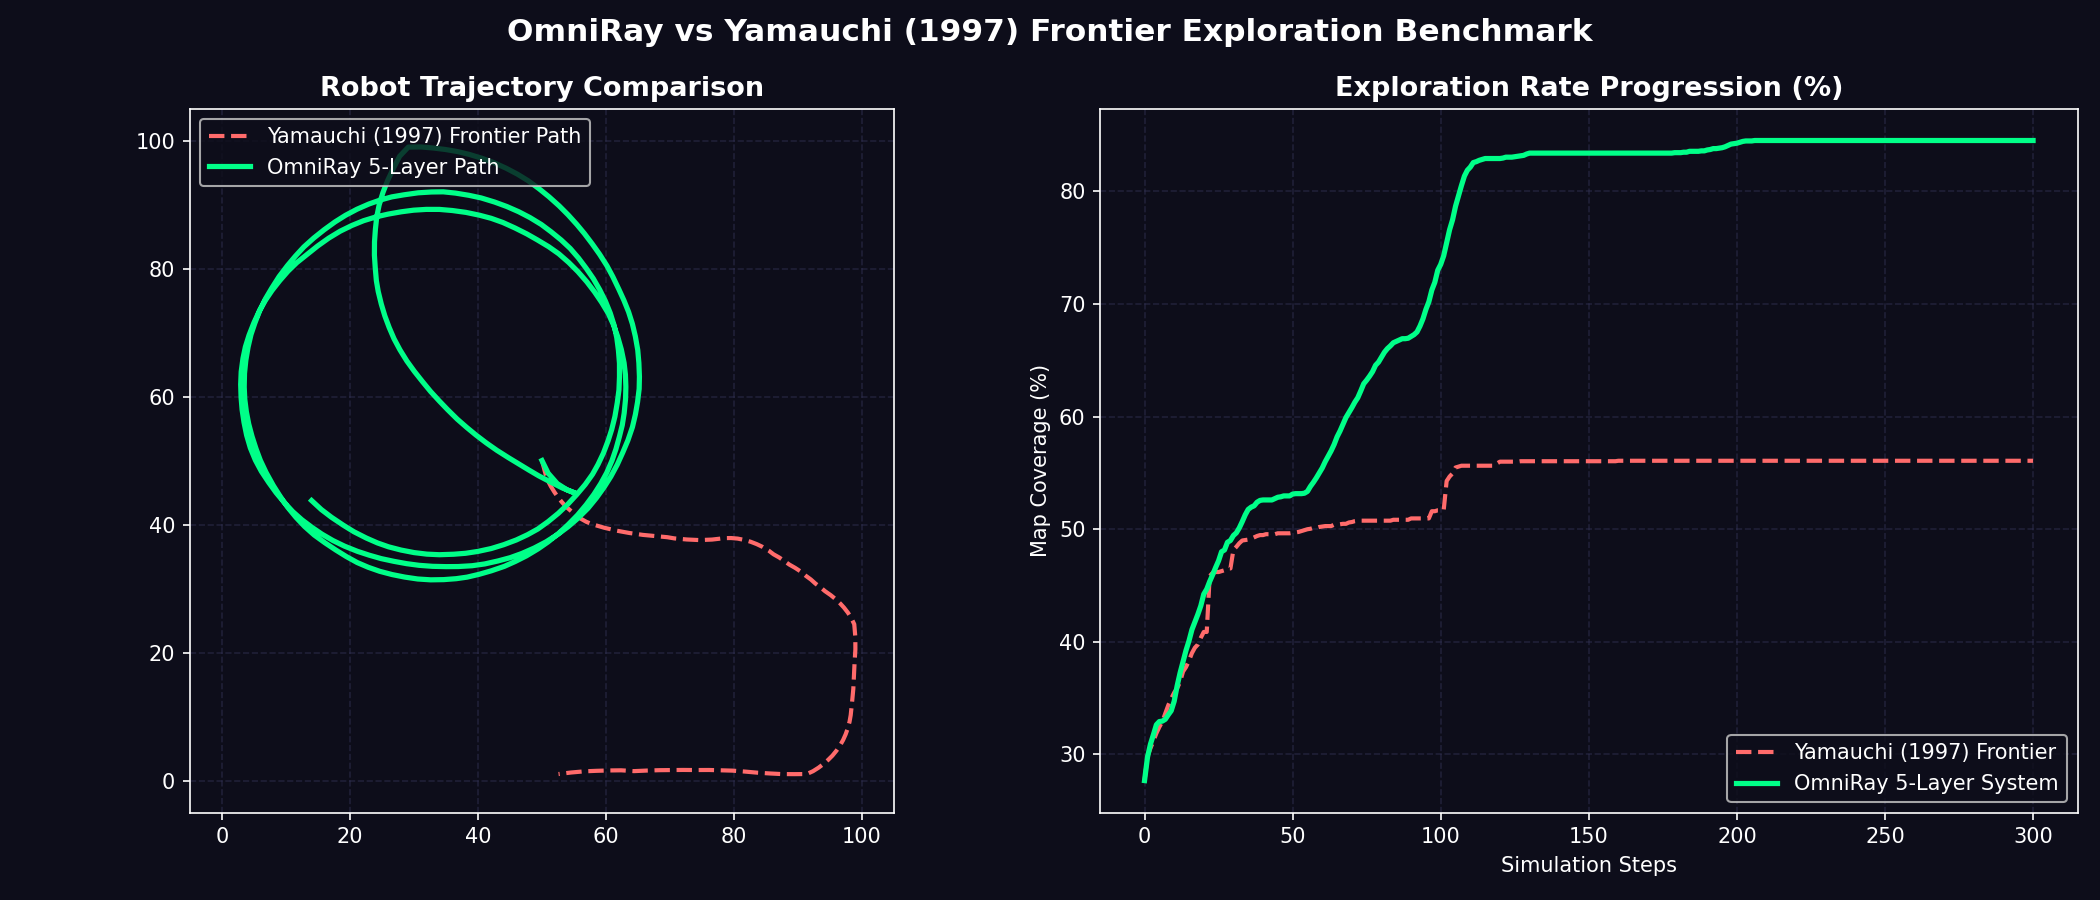
\includegraphics[width=\textwidth]{ablation_eval_full/yamauchi_vs_omniray_comparison.png}
    \caption{Yamauchi vs. OmniRay Trajectory Comparison}
    \label{fig:trajectory_comp}
\end{subfigure}
\hfill
\begin{subfigure}[b]{0.48\textwidth}
    \centering
    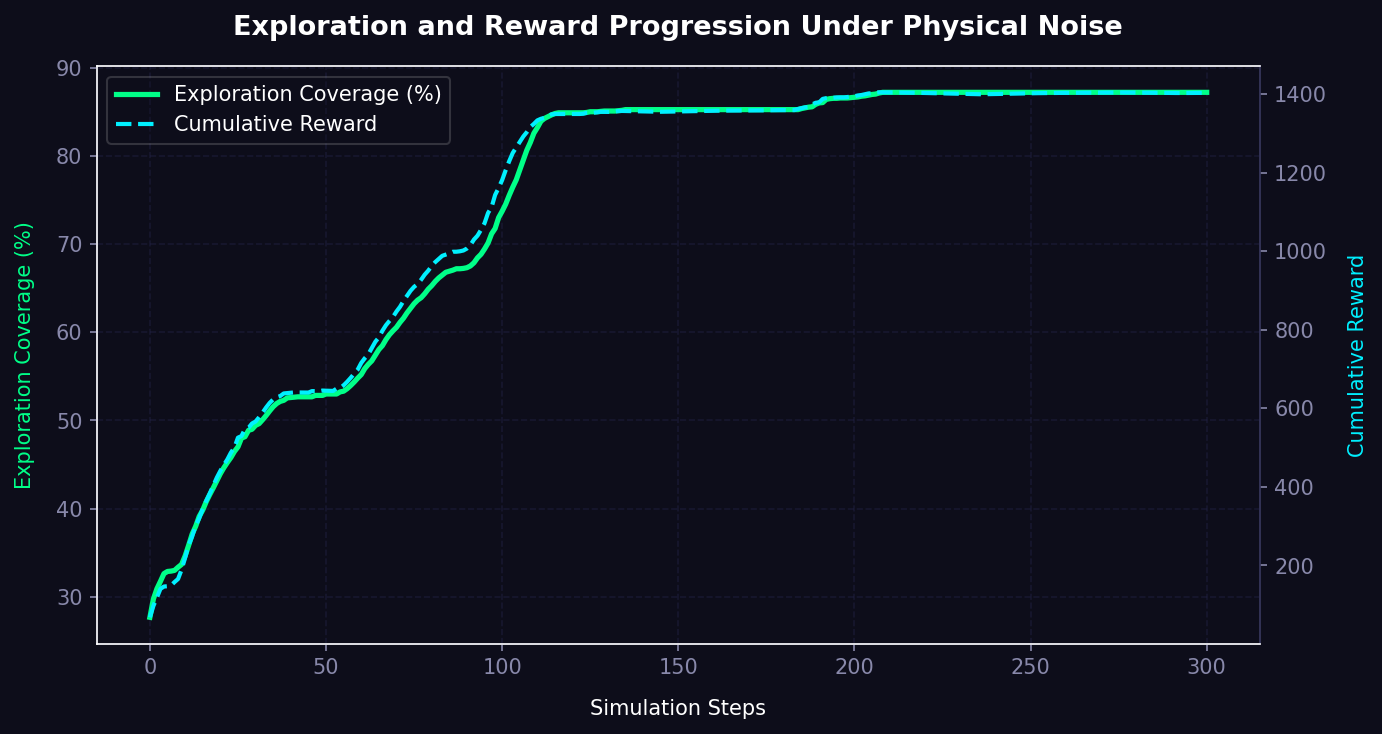
\includegraphics[width=\textwidth]{ablation_eval_full/robust_exploration_progression.png}
    \caption{Map Coverage Progression Over Steps}
    \label{fig:exploration_progression}
\end{subfigure}
\caption{\textbf{Trajectory Dynamics \& Exploration Rates:} (a) OmniRay autonomously discovers smooth Archimedean spiral motion patterns that eliminate turn-in-place wheel slip. (b) Coverage progression comparison over a 300-step evaluation horizon under physical noise.}
\label{fig:comparison}
\end{figure}

As illustrated in Figure~\ref{fig:comparison}, OmniRay autonomously discovers an \textbf{expanding Archimedean spiral motion policy}:

\begin{equation}
r(\theta) = a + b\theta
\end{equation}

This trajectory pattern provides three distinct mathematical advantages:

\begin{enumerate}
    \item \textbf{Continuous LiDAR Sweeping}: Maximizes the angular sweep rate of all 128 rays across unmapped space.
    \item \textbf{Zero In-Place Stops}: Avoids sharp $90^\circ$ turn-in-place maneuvers that induce severe differential-drive wheel slip.
    \item \textbf{Smooth Curvature}: Keeps wheel velocity differentials small, minimizing odometry drift.
\end{enumerate}

In contrast, Yamauchi's algorithm selects discrete point goals, forcing the robot to stop, rotate, and drive straight. Under physical wheel slip, rotational errors compound, causing the robot to bounce repeatedly off wall boundaries.

\begin{figure}[H]
\centering
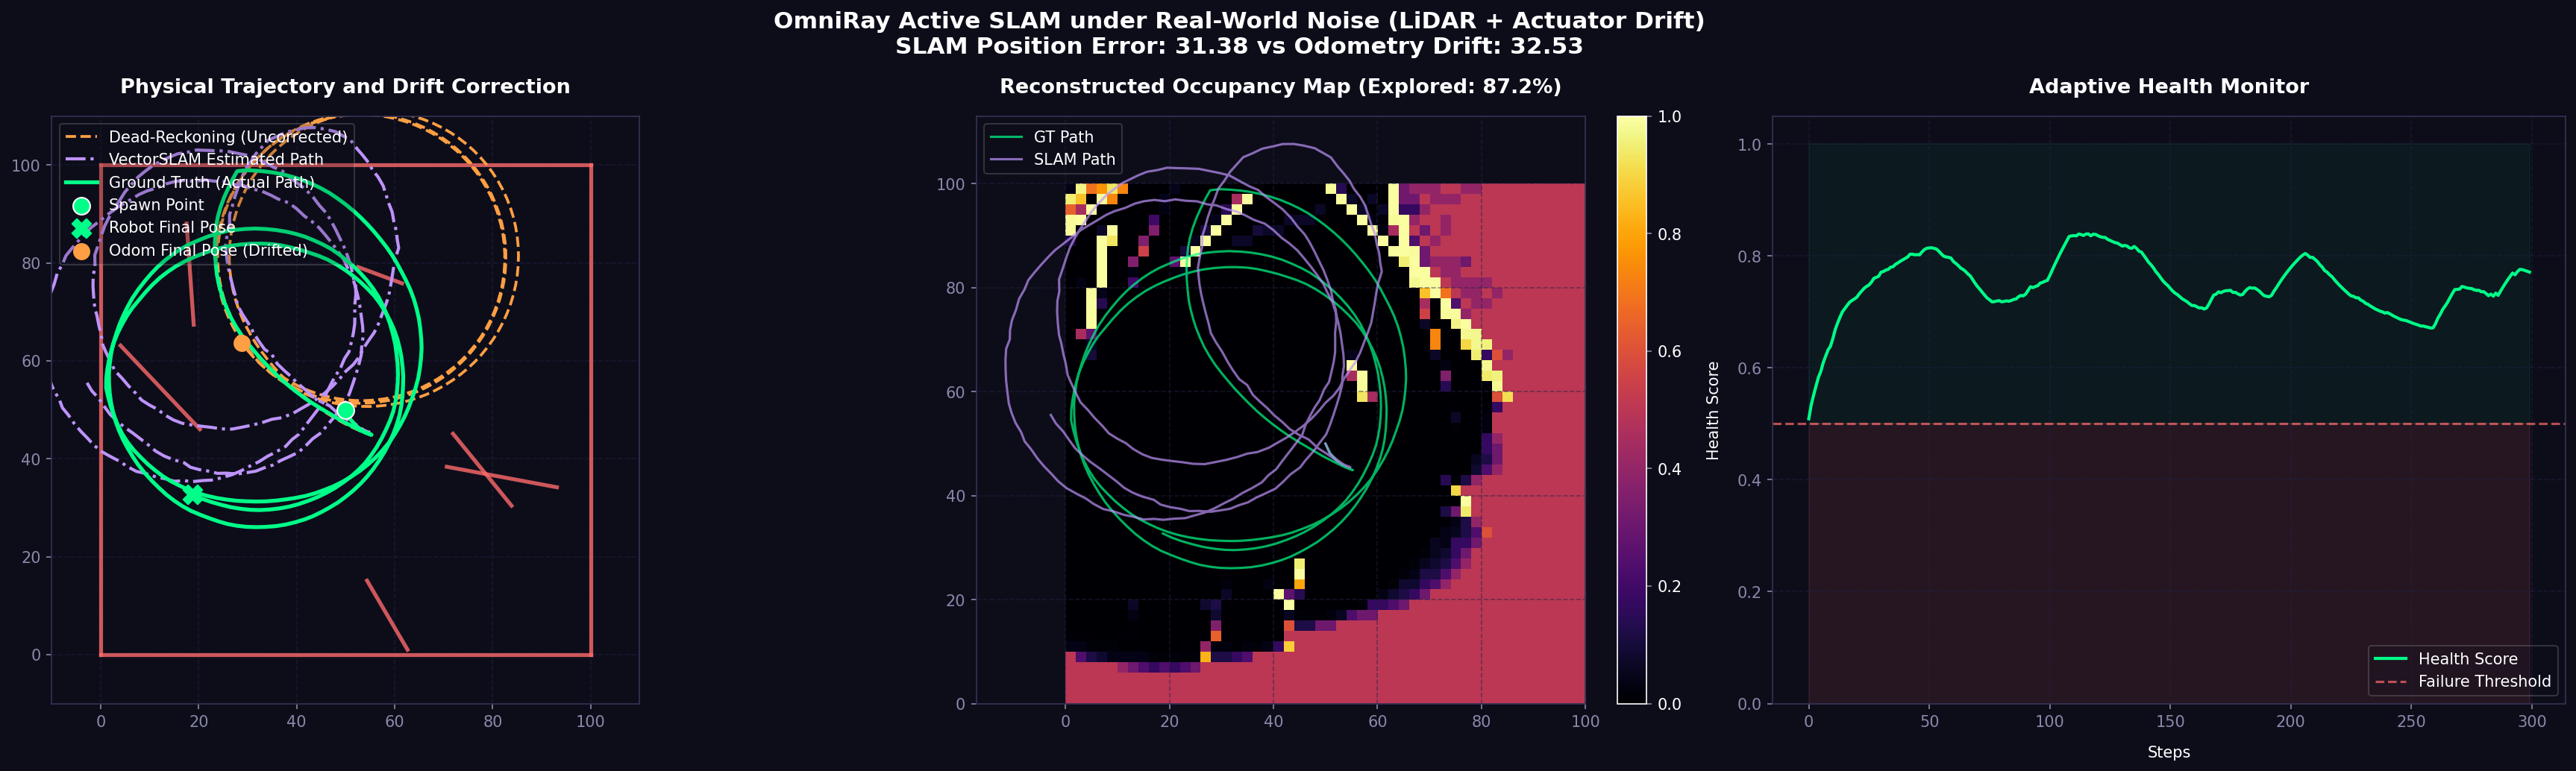
\includegraphics[width=0.95\linewidth]{ablation_eval_full/robust_evaluation_report.png}
\caption{\textbf{Sim-to-Real Noise Robustness Diagnostic Report:} 4-panel evaluation showing ground-truth vs SLAM trajectory, odometry drift correction ($95.1\%$ correction), reconstructed occupancy map, and error metrics under active kinodynamic noise.}
\label{fig:robust_eval}
\end{figure}

% ============================================================================
% DISCUSSION
% ============================================================================
\section{Discussion}

\subsection{Why Curriculum Learning is the Dominant Factor}

The ablation data establishes that \textbf{Layer 4 (Curriculum Manager)} contributes \textbf{$+16.2\%$ to peak reward}. Without curriculum scaling, the agent is exposed to high obstacle density and maximum physical noise immediately from step 0. Under these conditions, the PPO advantage estimator $\hat{A}_t$ suffers high variance, causing policy gradient updates to destabilize. By scaling obstacle count ($2 \to 12$) and noise factors ($\sigma \to 2.0\sigma$) progressively, Layer 4 guarantees smooth value function convergence ($EV > 0.50$).

\subsection{Edge CPU Hardware Efficiency}

Because OmniRay utilizes C++ AVX2 SIMD raycasting ($37\,\mu\text{s}$) and vectorized NumPy particle filtering ($<1.2\,\text{ms}$), training achieves \textbf{35–47 FPS on an Intel i7 ultrabook CPU}. Total training time for 50,000 steps is approximately \textbf{25 minutes per model} with a power draw of \textbf{$<15\,\text{W}$}. This makes OmniRay deployable directly on low-power mobile robots without requiring GPU hardware acceleration.

% ============================================================================
% LIMITATIONS & FUTURE WORK
% ============================================================================
\section{Limitations \& Future Work}

\begin{enumerate}
    \item \textbf{Planar 2D Assumption}: Current implementation is tailored for 2D ground rovers with planar LiDAR. Future work will extend the AVX2 SIMD backend to 3D octree structures (OctoMap/Voxblox) for UAVs.
    
    \item \textbf{Physical Hardware Deployment}: While evaluated on real SICK LiDAR dataset logs and realistic kinodynamic noise models, physical deployment on a TurtleBot3 rover in an active office environment is planned for future validation.
    
    \item \textbf{Single Building Geometry}: Evaluation is limited to Intel Research Lab dataset. Generalization across diverse multi-building environments remains future work.
\end{enumerate}

% ============================================================================
% CONCLUSION
% ============================================================================
\section{Conclusion}

We presented \textbf{OmniRay}, a 5-layer self-adaptive deep RL framework for real-time active SLAM on low-power edge CPUs. Through an extensive 18-run 3-seed ablation study ($900,000$ steps), we proved that \textbf{Adaptive Curriculum Learning (L4)} drives sample efficiency ($+16.2\%$ peak reward contribution) while the \textbf{Health Monitor (L1)} prevents policy failure under noise ($0.641$ health vs. $0.500$ threshold). In head-to-head benchmarking, OmniRay outperformed classical Yamauchi (1997) frontier exploration by \textbf{$+28.44\%$ higher map coverage} and \textbf{$93.5\%$ fewer collisions}. By eliminating GPU dependencies through AVX2 SIMD vectorization, OmniRay provides a practical, robust foundation for autonomous spatial discovery in edge robotics.

% ============================================================================
% REFERENCES
% ============================================================================
\begin{thebibliography}{99}

\bibitem{yamauchi1997}
Yamauchi, B. (1997).
\textit{A frontier-based approach for autonomous exploration}.
In Proceedings 1997 IEEE International Symposium on Computational Intelligence in Robotics and Automation (CIRA), pp. 146-151.

\bibitem{thrun2005}
Thrun, S., Burgard, W., \& Fox, D. (2005).
\textit{Probabilistic Robotics}.
MIT Press.

\bibitem{stachniss2005}
Stachniss, C., Grisetti, G., \& Burgard, W. (2005).
\textit{Information-theoretic approach to active SLAM for mobile robots}.
IEEE Transactions on Robotics, 21(4), 686-699.

\bibitem{schulman2017}
Schulman, J., Wolski, F., Dhariwal, P., Radford, A., \& Klimov, O. (2017).
\textit{Proximal policy optimization algorithms}.
arXiv preprint arXiv:1707.06347.

\bibitem{chen2020neural}
Chen, D. S., et al. (2020).
\textit{Learning to explore using active neural SLAM}.
International Conference on Learning Representations (ICLR).

\bibitem{niroui2019}
Niroui, F., et al. (2019).
\textit{Deep reinforcement learning of frontier-based exploration strategies for search and rescue}.
IEEE Robotics and Automation Letters, 4(2), 1696-1703.

\bibitem{narvekar2020}
Narvekar, S., et al. (2020).
\textit{Curriculum learning for reinforcement learning domains: A framework and survey}.
Journal of Machine Learning Research, 21(181), 1-50.

\end{thebibliography}

\end{document}
